\section{Project description}
The project description was written by A. Malthe-S{\o}renssen.\\
\\
Most of the worlds currently accessible hydrocarbon resources are found in tight rocks - rocks with permeabilities in the millidarcy range and with pore sizes in the nanometer range. The development of technologies for production from tight rocks have changed the energy landscape, making countries such as US self-sufficient with gas and possibly also with oil, and the estimates from the producable reserves of hydrocarbons in tight rocks are continuously increased as new methods are developed and new plays are discovered. However, we are now at a stage where technological and engineering methods have surpassed our basic scientific understanding of production from tight rock systems.\\
Tight rocks pose new scientific problems because of the small length-scales involved. Traditional oil plays are found in for example sand stone reservoirs with millimeter to micrometer sized pores. For such systems, standard hydrodynamics is a sufficient tool to understand, describe and predict fluid transport, even for multiphase systems. However, in tight rocks, typical pore sizes are in the range of tens to hundres of nanometers. For such systems, the finite size of the atoms and molecules that make out fluids and surfaces become important: The dielectric properties of water and surface charge distributions, the binding energies of the fluids to the surfaces, and the effects of surface shapes and irregularities on effective surface interactions become important. For example, the usual assumption in fluid mechanics of no-slip boundary conditions may no longer hold, the fluids may behave differently close to surfaces than in bulk, and for smaller pores the surface to volume ratio is larger than for larger systems, and for gases the mean free path may become comparable to the characteristic sizes of the porous medium. These effects introduce challenges in how to describe and model fluid flow and surface reactions in tight rocks.\\
We have initiated an activity in tight rocks to address tight-rocks-specific effects for enhanced hydrocarbon production and CO2 storage. A part of that initiative requires the development of better models to address fluid flow, both liquids and gases, in tight rocks geometries with a particular focus on shale systems. In this project, we will address fluid flow in tight rocks systems by developing models to address atomistic effects for dilute gases and water in hydrophilic systems. To do this we need different models spanning various length scales. To address the flow of dilute gases in complex geometries on nanometers to micrometer length scales we will develop a method called Direct Simulation Monte Carlo (DSMC), that models a gas through effective particles that collide with other gas particles with stochastic collision rules that conserves momentum and that interacts with surfaces through special reflection rules that can be tuned using for example theoretical, experimental or atomic scale modeling results. Such models have proven useful to address dilute gas flows in regular geometries, such as for tube and channel flows, but we need very general tools to address the complex geometries of tight rocks system as found in experimental, tomographical studies. To supplement the modeling of dilute gases, we will also need methods to address the dynamics and flow of water in small pores using atomic scale models. In that case we need to model specific materials, and we have access to a very good molecular dynamics (MD) model for the interaction between water and silicates that we plan to develop and use to address fluid flow in nanoscale geometries. In this project we will develop both a DSMC and a MD model to address gas and liquid flow in tight rocks system.
\section{Shale gas extraction}
Shale gas is a type of natural gas trapped in shales - low permeability tight rocks with pore sizes at the nanometer scale. In these reservoirs, the gas is stored inside already existing pore networks or adsorbed onto organic matter. To be able to extract gas from such materials, fractures are generated to increase the permeability so the production rate approaches an adequate level. Today we usually use horizontal drilling; we drill from the earth surface, vertically, until we reach the shale formation, before the drilling is continued horizontally inside the shale, see figure \ref{fig:shale_gas_extraction}.
\begin{figure}[h!]
\begin{center}
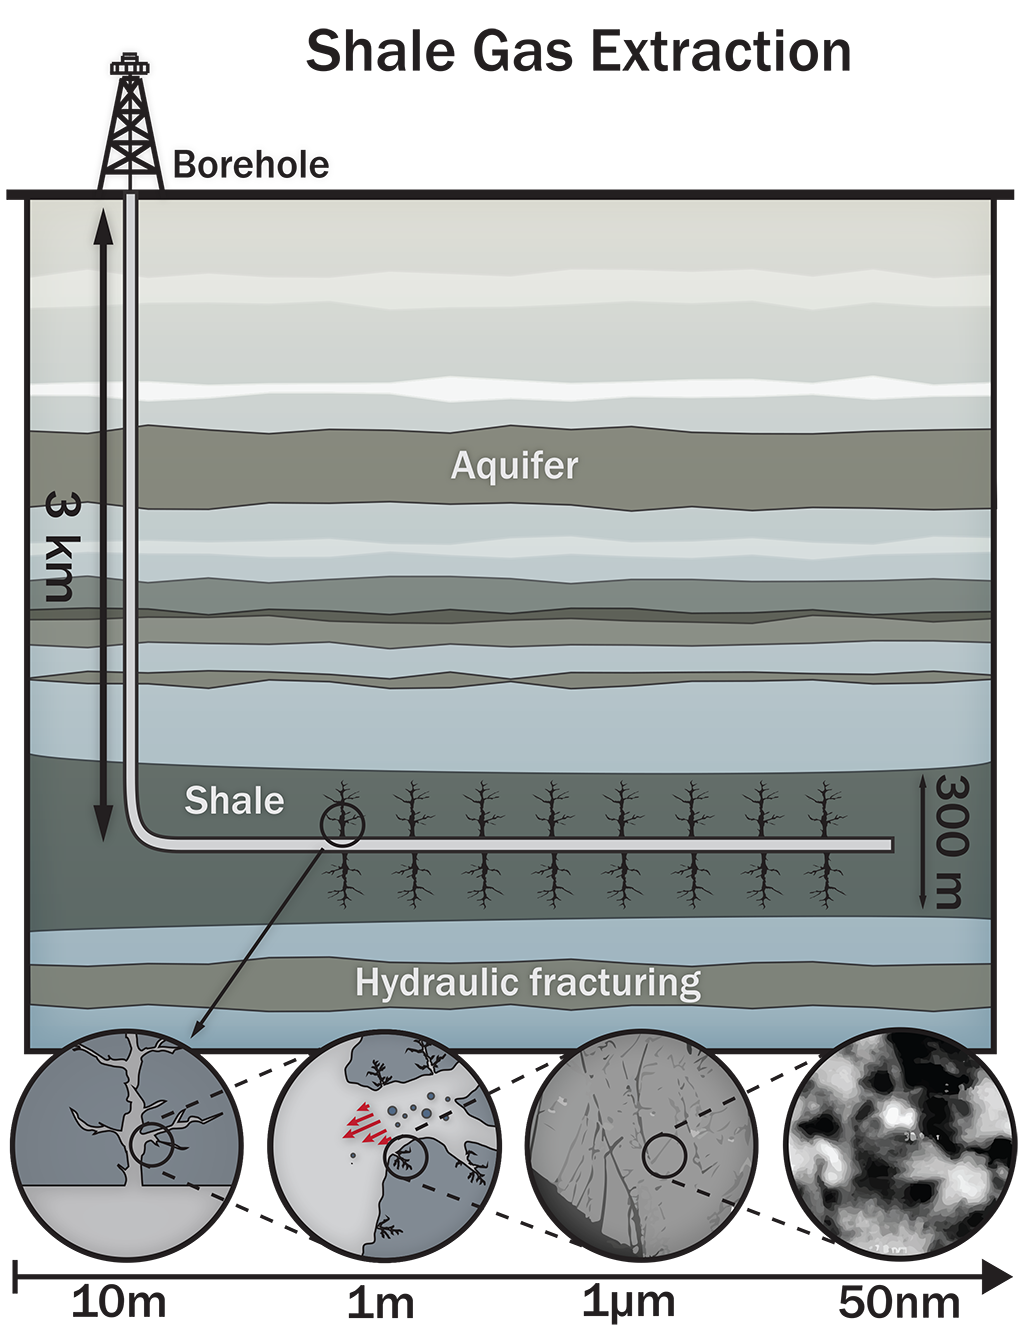
\includegraphics[width=0.7\textwidth, trim=0cm 0cm 0cm 0cm, clip]{figures/shale_gas_extraction.png}
\end{center}
\caption{Shale gas extraction principles. Hydraulic fracturing cracks the shales, releasing the trapped gas. In this process, physical phenomena on all length scales from nanometers to meters may be relevant. The production occurs in nanometer pores whereas the gas gathers in the larger fracture networks to the final drilling hole the gas flows through to the earth surface. }
\label{fig:shale_gas_extraction}
\end{figure}
The fractures are generated by hydraulic fracturing - millions of liters of water are injected with an extreme pressure cracking the shales. Proppants - small, usually spherical, ceramic materials - are mixed into the water keeping the fractures open even after the pressure is released. The gas then flows from the nanosized pores into the fracture network through very small channels. Even after the hydraulic pressure is decreased, the pressure inside the shale formation is higher than the surface pressure making the gas flow through the drilling hole to the earth surface.\\
The whole process of shale gas extraction then needs to couple physics at length scales covering more than 10 orders of magnitude. In this thesis, we focus on the smallest scale from which the gas is produced. 

\section{Goals}
\renewcommand{\thesubsection}{\thesection.\alph{subsection}}
To be able to study flow in systems similar to the fractured networks, we have chosen a set of goals to be achieved during the work with this thesis. Achieving these goals will combined lead to a solid base understanding of how the physics of fluids works at the nanometer scale, as well as having developed great tools for further study. The goals are twofold, software development and applications of the software. 
\subsection{Develop a three-dimensional parallel DSMC model}
\label{goal:dsmc_1}
The DSMC model has been used for the past 50 years to study flow of dilute gases in systems where the mean free path is of the same order as a characteristic size of the geometry. Having an implementation of this model will allow us to simulate flow in systems with channels so small that continuum mechanics do not longer produce correct physical behavior. The implementation needs to be parallelized for large-scale parallel machines.
\subsection{Develop methods to model arbitrary 3d geometries}
\label{goal:dsmc_2}
Important systems for theoretical purposes are for example cylinders or other simple, mathematically well-described geometries. They can in many cases have analytical solutions and be excellent test cases for a more general numerical model. However, real fracture networks are usually defined by a complicated geometry with no closed form mathematical description. We therefore need to find a way to represent arbitrary geometries allowing us to measure flow properties in more realistic systems.
\subsection{Develop a three-dimensional parallel MD model}
\label{goal:md_1}
Different surface materials may interact very differently with the same fluid. Take for example water. Some surfaces are \textit{hydrophilic}, which means that they attract water, whereas \textit{hydrophobic} materials tend to repel water. This will of course affect how the fluid flows through a system. The DSMC model is a particle model that performs stochastic collisions with collision rules that use parameters depending on the combination of the specific surface material and fluid substance. With a good MD model, we can both study flow in small systems and compute the gas-surface parameters we need in DSMC. 
\subsection{Develop custom 3d visualization tools for large particle data sets}
\label{goal:vis}
Both models produce time trajectories of the particles from a given initial state. The output data is a set of particle positions which can be visualized to learn more about the fluid dynamics. By building such visualization tools from scratch, we can overcome the drawbacks that are in the already available free software (these drawbacks are discussed later) and create custom features that satisfy our needs. 

\subsection{Study flow and dynamics of water in simple nanoscale silicates}
\label{goal:md_2}
With an advanced atomic potential in MD, we can study how water flows in nanoscale silicates \cite{vashishta1990interaction}. Such a potential can for example be used to study how hydroxyl groups on the surface of the silicate affect the water flow. This can also be used to produce gas-surface parameters that enable us to study larger scale systems with the same statistical surface behavior as water in silicates. 

\subsection{Gain insight with correction factors for permeabilities in nanoporous media}
\label{goal:knudsen}
It is well known from experiments that the measured permeabilities in nanoporous media can be two orders of magnitues higher than the theoretical predicted values. Klinkenberg explained this effect by the fact that the fluid can have a non-zero velocity near the boundaries\cite{klinkenberg1941permeability}. Slip velocity leads to a correction to the theoretically predicted permeability. We will study flow in different nanoporous media to see how well these corrections predicts the permeability in the stochastic DSMC model as well as the MD model for systems with different pore sizes covering two orders of magnitudes. 
\renewcommand{\thesubsection}{\thesection.\arabic{subsection}}

\section{The structure of this thesis}
This document is arranged in five parts. Chapter \ref{chap:theory_of_fluids} opens with a brief discussion about the theory of fluid mechanics. We discuss how the continuum approach in standard hydrodynamics breaks down for dilute gases in nanoporous media, and what the current theory has to offer in predictions of the permeability. The largest subject of this study is the DSMC model in part \ref{part:dsmc}. It begins with an introduction to kinetic theory in chapter \ref{chap:kinetic_theory} which we use in \ref{chap:dsmc} when we introduce the DSMC model. The implementation of the model is explained in chapter \ref{chap:dsmc_implementation} with the numerical results presented in \ref{chap:dsmc_results}.\\
In part \ref{part:md}, we discuss MD, the second model we have studied. We begin by introducing the theory behind MD in chapter \ref{chap:md} with the implementation in chapter \ref{chap:md_implementation}. The results are presented in chapter \ref{chap:md_results}. The final part is concerned with our desire of creating a custom 3d visualization tool that we can use to visualize the simulations we perform with both models. We start by a brief introduction to OpenGL in chapter \ref{chap:opengl} where we explain graphics programming and how the graphics card can be used to draw geometrical models on a computer screen. In chapter \ref{chap:particle_visualizer} we explain how to use advanced shaders in the rendering pipeline to render the time evolution of tens of millions of atoms on the screen. We also discuss the marching cubes algorithm that is used to render the geometry used in a DSMC simulation.

\section{My contribution}
In every thesis, as in any other scientific work, the foundation of the prduced content is results from previous work. It should be clear what new ideas the author has contributed with. This could for example be new theoretical calculations, models, algorithms or tools that has been developed. Since a master thesis is a larger document containing more information than just the new contributions, it might be less obvious which parts that are the unique work of the author. Such a document deserves its own section highlighting these parts.\\
Both models we have studied in this thesis have been programmed and implemented from scratch. A total of approximately 20000 lines of code have been written in C{}\verb!++! and \verb!Python!. Writing everything from scratch provides a great insight in both models, especially from a numerical perspective, since every detail of the implementation has to be understood. In this section we briefly discuss the contributions by the author. This section is not meant to be an introduction to any of the concepts, so it is assumed that the reader is familiar with the models at the time of reading. If this is not the case, everything in this section should be clear after reading about both models and the visualization program in chapters \ref{chap:dsmc}, \ref{chap:dsmc_implementation}, \ref{chap:md}, \ref{chap:md_implementation} and \ref{chap:opengl}.
\subsection{Direct Simulation Monte Carlo}
In the DSMC model, we need to represent the geometry of the system (of which the fluid is confined in). This method has to be fast, scalable (for parallelizing) and general so that we can represent an arbitrary geometry. To be able to perform collisions between the surface and the particles, the surface needs to have well defined normal and tangent vectors in every available collision point. The author has developed a voxelation model with a new algorithm to compute the normal and tangent vectors based on the neighboring voxels. This gives a smoother effective surface than just voxel values. We discuss this model in detail in section \ref{sec:dsmc_complex_geometries}.
\subsection{Molecular Dynamics}
The MD code is a standard, but remarkably efficient code using the Lennard-Jones potential. The code structure and parallelization technique is based on what is teached at the University of Southern California \footnote{See \url{http://cacs.usc.edu/education/cs596/ParallelMD-VG.pdf} for details.}. In section \ref{sec:md_complex_geometries} we discuss that we want to simulate a fluid in an arbitrary geometry with the MD code. The author has developed a simple, but very promising model of a solid that allows a set of atoms to behave as a solid, vibrating about their equilibrium point while interacting with the fluid with realistic atomic forces. In addition, with an applied thermostat on these atoms, we are able to drain the system for energy which is a necessity when we induce flow in the system by adding a constant force as described in section \ref{md:pressure_driven_flows}. The details of this model is discussed in section \ref{sec:md_complex_geometries}.
\subsection{Visualization}
The free visualization software available, such as VMD and Ovito, are great tools for studying data sets from atomic or molecular models. There are two significant drawbacks the author has noticed; the camera control and performance. In both of these programs, the camera is looking towards a point, usually in the center of the system, whereas the mouse controls the rotation around this point. To be able to study different parts of the system in detail, one could want to control the camera as in a first person shooter game. The author has, together with Svenn-Arne Dragly, developed visualization tools allowing us to visualize up to 100 million atoms simultaneously with decent frame rate with the camera control described above. In chapter \ref{chap:opengl} we discuss how to make full use of \textit{geometry shaders}, which allow us to render the spheres representing the atoms on the Graphical Processing Unit (GPU). 